\documentclass{article}

% Language setting
% Replace `english' with e.g. `spanish' to change the document language
\usepackage[english]{babel}

% Set page size and margins
% Replace `letterpaper' with `a4paper' for UK/EU standard size
\usepackage[letterpaper,top=2cm,bottom=2cm,left=3cm,right=3cm,marginparwidth=1.75cm]{geometry}
\usepackage{bm}

% Useful packages
\usepackage{amsmath}
\usepackage{amssymb}

\usepackage{algorithm}
\usepackage{algpseudocode}
\usepackage{appendix}

\usepackage{graphicx}
\usepackage[colorlinks=true, allcolors=blue]{hyperref}

\usepackage{subcaption}

\usepackage{tikz}

% Costume Style Begin
\usepackage{enumitem}
% Costume Style End

% Operator Declaration Begin

% Operator Declaration End

\title{SUSTech CS324 2024 Spring Assignment 1 Report}
\author{12110304 Chunhui XU}

\begin{document}
\maketitle

\section{Part 1}

In this part, I need to create a simple perceptron to complete a two-classification problem. But before start, I will provide some information about perceptron in this Part \textbf{refer from our tutorial materials}.

\subsection{Problem Analysis}

\subsubsection{Simple Introduction}

A perceptron takes multiple input values, each multiplied by a weight, sums them up, and produces
a single binary output based on whether the sum is above a certain threshold.

In my code implementation, I simply insert a new column as the bias value.


\subsubsection{Mathematical Model}

The perceptron decision is based on these formulas:
$$
    f(x) = sign(w\cdot x+b)
$$

$$
sign(x)=
\left\{
    \begin{aligned}
        +1 && \text{if $x \geq 0$}\\
        -1 && \text{if $x < 0$}
    \end{aligned}
\right.
$$

Components of a Perceptron:

\begin{itemize}
    \item Inputs (x): The features or data points provided to the perceptron.
    \item Weights (w): Coefficients determining the importance of each input.
    \item Bias (b): An extra input (always 1) with its own weight, allowing the activation function to shift,
fitting the data better.
    \item Activation Function(sign function): Decides whether the neuron should activate, typically a
step function for basic perceptrons
\end{itemize}

\subsubsection{Loss Function}

We need to design a loss function to compute the model loss, 

% \begin{align*}

% \end{align*}

\begin{align*}
    L_{1}(w,b) &= \sum_{i=1}^{N}-y_{i}*f(x_{i}) \textbf{ when } y_{i}*f(x_{1})<0 \\
               &= \sum_{i=1}^{N}-y_{i}*sign(w*x_{i}+b) \textbf{ when } y_{i}*sign(w*x_{i}+b <0\\
    L_{2}(w,b) &= \sum_{i=1}^{N}\frac{1}{||w||}|w*x_{i}+b| \textbf{ when } y_{i}*(w*x_{i}+b)<0\\
               &= -\frac{1}{||w||}\sum_{i=1}^{N}y_{i}*(w*x_{i}+b) \textbf{ when } y_{i}*(w*x_{i}+b)<0
\end{align*}

Obviously, the first function just compute the number of misclassified points, it cannot be differentiated, so I choose $L_2$ as my loss function, which expresses the total distance
from the misclassified point to the hyperplane $S$.

And we can ignore this coefficient $\frac{1}{||w||}$, the loss function is:
$$
L_{3}(w,b)=-\sum_{i=1}^{N}y_{i}*(w*x_{i}+b)\ \text{ when } y_{i}*(w*x_{i}+b)<0
$$

In this way, the derivation of Loss function is:
\begin{align*}
    \nabla_{w}L(w,b) &= -\sum_{x_{i} \in M}y_{i}x_{i}\\
    \nabla_{b}L(w,b) &= -\sum_{x_{i} \in M}y_{i}
\end{align*}

\subsubsection{Gradient Descent}

We need to get the gradient descent equation, that is

$$
b=a-\gamma\nabla f(a)\\
$$

where $\gamma$ is the learning rate (usually 0.01).

\subsubsection{Types of Gradient Descent}
\begin{itemize}
    \item \textbf{Batch Gradient Descent (BGD)}: In batch gradient descent, model parameters are updated after computing the gradient of the cost function with respect to the entire training data set. It involves computing the gradient of the cost function over the entire dataset at each iteration, which can be computationally expensive for large datasets.

    \item \textbf{Stochastic Gradient Descent (SGD)}: Unlike batch gradient descent, stochastic gradient descent updates model parameters after computing the gradient of the cost function for only one randomly selected training example at a time. Compared to batch gradient descent, this method is computationally cheaper, especially for large datasets, since it only requires computing the gradient for a single example in each iteration.

    \item \textbf{Mini-Batch Gradient Descent}: Mini-batch gradient descent combines the advantages of batch gradient descent and SGD, updating model parameters in each iteration based on a small random subset of the training data set.
    This method strikes a balance between the computational efficiency of SGD and the stability of batch gradient descent.
\end{itemize}

\subsubsection{The “standard” algorithm}
Given a training set $D = \{(x_{i},y_{i})\}, x_{i}\in \mathbb{R}^{N}, y_{i}\in \{-1,1\}$
\begin{enumerate}
    \item Initialize $w=0\in\mathbb{R}^{n}$
    \item For epoch $= 1 \cdots T:$
        \begin{enumerate}
            \item Compute the predictions of Perceptron of the whole training set
            \item Compute the gradient of the loss function with respect to $w$:
            $$gradient = -\frac{1}{N}\sum(x_{i} \cdot y_{i}), for\ sample_{i}:p_{i}*y_{i}<0$$
            where $p_{i}$ is $i$ th prediction, $y_{i}$ is the related ground truth of sample $i$, $N$ is the number of misclassified points
            \item Update $w \leftarrow w - lr * gradient$
        \end{enumerate}
    \item Return $w$
\end{enumerate}

\subsection{Results Display}

In Part1, I insert a bias column, so it's no need to generate symmetric mean value.

\subsubsection{Data Feature}

I generate 3 test example, the Table \ref{tab:p1feat} show the detailed information. They are the test ID, the mean of positive and negative samples, and the covariance of positive and negative samples.

\begin{table}[!ht]
\centering
\caption{Data Set Feature}
\label{tab:p1feat}
\begin{tabular}{|l|c|c|c|c|c|} \hline
ID & Mean Pos & Mean Neg & Cov Pos & Cov Neg   \\ \hline
1 & [3, 3] & [15, 15] & [[2,0], [0,2]] & [[2,0], [0,2]] \\ \hline
2 &	[3, 3] & [6, 6] & [[10,0], [0,10]] & [[10,0],[0,10]] \\ \hline
3 &	[3, 3] & [4, 4] & [[2,0], [0,2]] & [[2,0], [0,2]] \\ \hline
\end{tabular}
\end{table}

\subsubsection{Default Parameters}

\begin{itemize}
    \item \texttt{n\_inputs}: $2$, number of inputs
    \item \texttt{max\_epochs}: $100$, maximum number of training cycles
    \item \texttt{learning\_rate}: $0.01$, magnitude of weight changes at each training cycle
\end{itemize}

\subsubsection{Data Visualization}

\begin{figure}[!ht]
  \centering
  \begin{subfigure}[b]{0.45\textwidth}
    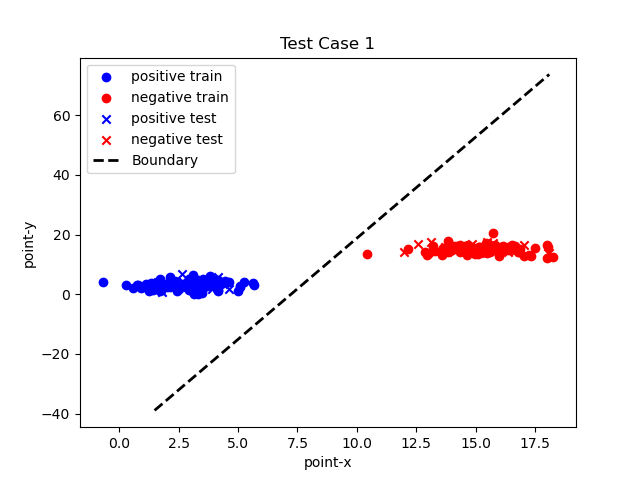
\includegraphics[width=\textwidth]{img/Part1/test1_data.png}
    \caption{Test case 1 Data}
  \end{subfigure}
  \begin{subfigure}[b]{1\textwidth}
    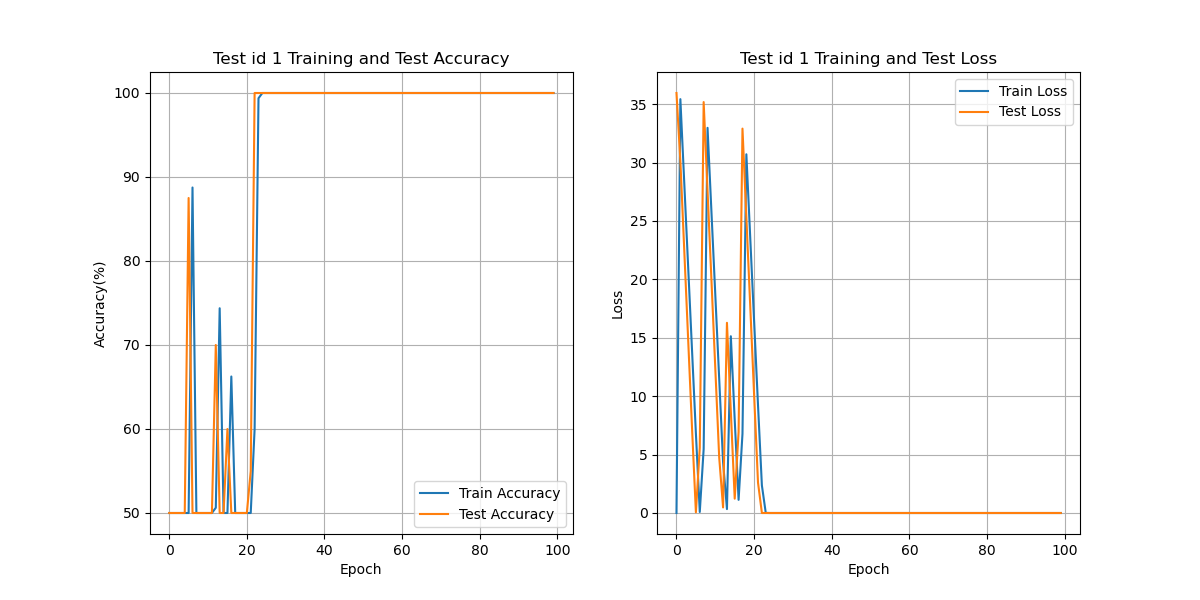
\includegraphics[width=\textwidth]{img/Part1/test1_curve.png}
    \caption{Test case 1 Accuracy and Loss}
  \end{subfigure}
  \caption{Test Case 1}
  \label{fig:p1test1}
\end{figure}



Figure \ref{fig:p1test1},  show us an example of data visualization for the data and train. 

Also, you can check Figure \ref{fig:p1test2}, Figure \ref{fig:p1test3} in Appendix section. 

\subsection{Results Analysis}

\subsubsection{Data Feature Analysis}

Actually, the 3 test case corresponding to 3 different situations:

\begin{enumerate}
    \item The mean difference is large, and the respective variances are small.
    \item The variances are both large.
    \item The mean difference is small.
\end{enumerate}

\subsubsection{Training Loss and Accuracy Analysis}

By comparing the three pictures, we can find that when the mean difference between positive and negative samples is large and their respective variances are small, the classification is more accurate and the training results are better.

The latter two case lead to two different situation:

\begin{itemize}
    \item \textbf{The variances are both large}: Although the difference between the means may be large enough, excessive variance will cause the data to deviate more from the mean. This will lead to a possible situation: positive and negative samples are each generated near the mean of the other party.
    \item \textbf{The mean difference is small}: In this case, the points of the two types of samples will be too close. In this case, the points of the two types of samples will be mixed together, making it difficult to find a suitable way to classify them accurately.
\end{itemize}

In both cases, one type of data acts like a "spy" masquerading as the other's sample points. it is easy to be predicted by Perceptron as the other party's sample point during training, conflicting with its own label, causing training 
 confusion and leading to problems.

Intuitively, this is because the latter two case will cause the possible areas of positive and negative sample points to overlap too high, making it difficult (or even impossible) to find a decision boundary to completely separate the two samples.

As training data continues to increase, it does not improve Perceptron's training efficiency. Instead, it continues to bring confusing and misleading information.

This results in Perceptron constantly adjusting its weight and bias to fit the training data during the training process, and making it difficult to converge to a stable value. So we can see that, the loss value and accuracy fluctuates wildly in case 2 and 3. Because the model cannot converge in a better direction during the training process, but may become worse due to misleading data.

Only data like 1 that can find effective decision boundary can be trained to achieve higher accuracy. Understanding from the images means that a boundary can be found to completely separate the two types of data.

\subsection{Simple Conclusion}

In this part, I implemented a Perceptron. Starting with some relatively simple methods of forward propagation, back propagation and gradient descent, I gained a basic understanding of the deep learning methodology.

\section{Part 2}


\subsection{Problem Analysis}

In this part, I need to create a a multi-layer perceptron(MLP) by Numpy, generate a given dataset and do the classification problem correctly.

\subsubsection{Simple Introduction}

In the second part, I use scikit-learn package and generate by \texttt{make\_moon} function. Then, I create a dataset of 1000 two-dimensional points. Let $S$ denote the dataset, i.e., the set of tuples $\{(x^{(0),s}, t^{s})\}_{s=1}^{S}$, where $x^{(0),s}$ is the $s$-th element of the dataset and $t^{s}$ is its label. And I need to use \texttt{OneHotEncoder} to encode the label.

After that, I need to implement the MLP and make correct classification for this problem.

\subsubsection{MLP Structure}

Let $d_{0}$ be the dimension of the input space and $d_{n}$ the dimension of the output space. The network I build have $N$ layers (including the output layer). In particular, the structure will be as follows:

\begin{itemize}
    \item Each layer $l = 1, \cdots , N$ first applies the affine mapping
    $$
        \tilde{x}^{(l)} = W^{(l)}x^{(l-1)}+b^{(l)}
    $$
    where $W^{(l)} \in \mathbb{R}^{d_{l}\times d_{(l-1)}}$ is the matrix of the weight parameters and $b^{(l)} \in \mathbb{R}^{d_{l}}$ is the vector of biases. Given $\tilde{x}^{(l)}$, the activation of the $l$-th layer is computed using a ReLU unit
        $$        
            x^{(l)} = \max(0,\tilde{x}^{(l)})
        $$
    \item The output layer (i.e., the $N$-th layer) first applies the affine mapping
        $$
            \tilde{x}^{(N)} = W^{(N)}x^{(N-1)} + b^{(N)}
        $$
    and then uses the softmax activation function (instead of the ReLU of the previous layers) to compute a valid probability mass function (pmf)
        $$
            x^{(N)} = \text{softmax}(\tilde{x}^{(N)}) = \frac{\exp(\tilde{x}^{(N)})}{\sum_{i=1}^{d_{N}}\exp(\tilde{x}^{(N)})_{i}}
        $$
    Note that both max and exp are element-wise operations.
    \item Finally, compute the cross entropy loss L between the predicted and the actual label,
        $$
            L(x^{(N)},t) = -\sum_{i}t_{i}\log{x_{i}^{(N)}}    
        $$
\end{itemize}

Particularly, in this assignment, there is only one hidden layer, the final structure is:

\begin{enumerate}
    \item $2$ input
    \item $2 \rightarrow 20$ Linear Layer
    \item $20 \rightarrow 20$ ReLU Layer
    \item $20 \rightarrow 2$ Linear Layer
    \item $2 \rightarrow 2$ Softmax Layer
    \item Output and Cross Entropy loss function
\end{enumerate}

\subsubsection{Default Parameters}

\begin{itemize}
    \item \texttt{dnn\_hidden\_units}: $[20]$, comma separated list of number of units in each hidden layer
    \item \texttt{learning\_rate}: $1\mathrm{e}^{-2}$, learning rate for optimization
    \item \texttt{max\_steps}: $1500$, number of epochs to run trainer
    \item \texttt{eval\_freq}: $10$, frequency of evaluation on the test set
\end{itemize}

\subsection{Forward and Backward Propagation Functions}

\subsubsection{Linear Layer}

Forward propagation:

$$
z = Wx + b
$$

\begin{itemize}
    \item $W$: weight matrix
    \item $x$: input vector
    \item $b$: bias vector
\end{itemize}

Backward propagation:

$$ \frac{\partial L}{\partial W} = \frac{\partial L}{\partial z} x^T $$
$$ \frac{\partial L}{\partial b} = \frac{\partial L}{\partial z} $$
$$ \frac{\partial L}{\partial x} = W^T \frac{\partial L}{\partial z} $$


\begin{itemize}
    \item $L$: The Loss function
    \item $\frac{\partial L}{\partial z}$: gradient of the loss with respect to the linear layer output
\end{itemize}


\subsubsection{ReLU Layer}

Forward propagation:

$$ y = \max(0, x) $$

\begin{itemize}
    \item $x$: input vector
\end{itemize}

Backward propagation:

$$
grad(x)=
\left\{
    \begin{aligned}
        1 && \text{if $x \geq 0$}\\
        0 && \text{if $x < 0$}
    \end{aligned}
\right.
$$

$$ \frac{\partial L}{\partial x} = \frac{\partial L}{\partial y} \cdot grad(x) $$

\subsubsection{Softmax Layer}

Forward propagation:

$$ \hat{y}_i = \frac{e^{z_i}}{\sum_{j=1}^{K} e^{z_j}} $$

\begin{itemize}
    \item $z_i$: $i$-th element of the input vector
    \item $K$: number of classes, that is $2$
\end{itemize}

Backward propagation:

The backward pass for softmax is often directly integrated with CrossEntropy for simplicity.

\subsubsection{Cross-entropy Loss}

Forward propagation:
$$ L = -\sum_{i=1}^{K} y_i \log(\hat{y}_i) $$

\begin{itemize}
    \item $y_i$: true label (one-hot encoded)
    \item $\hat{y}_i$: predicted probability for class $i$
\end{itemize}

Backward propagation:
$$ \frac{\partial L}{\partial z_i} = \hat{y}_i - y_i $$

\begin{itemize}
    \item  $y_i$: true label (one-hot encoded)
\end{itemize}

\subsection{Results and Display}

\subsubsection{Data Visualization}

Figure \ref{fig:p2sample} show the visualization of the whole data set. $1000$ positive data and $1000$ negative data.

\begin{figure}[!ht]
    \centering
    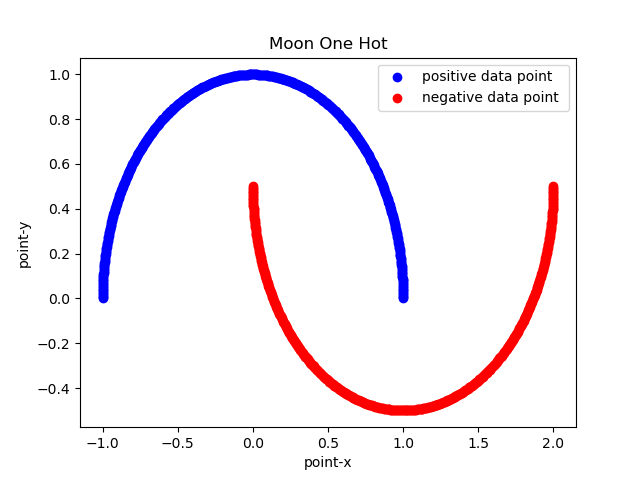
\includegraphics[width=0.6\textwidth]{img/Part2/sample_data.png}
    \caption{Moon Sample Data}
    \label{fig:p2sample}
\end{figure}

\subsubsection{My Additional parameters}

\begin{itemize}
    \item \texttt{batch\_size}: Positive value for Batch Gradient Descent and negative value for Mini-BGD (absolute value as batch size).
\end{itemize}

\subsubsection{Test Figure}

In our training, epoch is given and fixed, which means that the smaller the batch size, the more iterations are required, and large batches of parallel calculations are lost, which may take longer time.

Figure \ref{fig:p2batch1}, \ref{fig:p2batch10}, \ref{fig:p2batch100}, \ref{fig:p2batch800} show SGD, batch size 10, 100, 800 for 1500 epoch respectively.

\begin{figure}[!htbp]
    \centering
    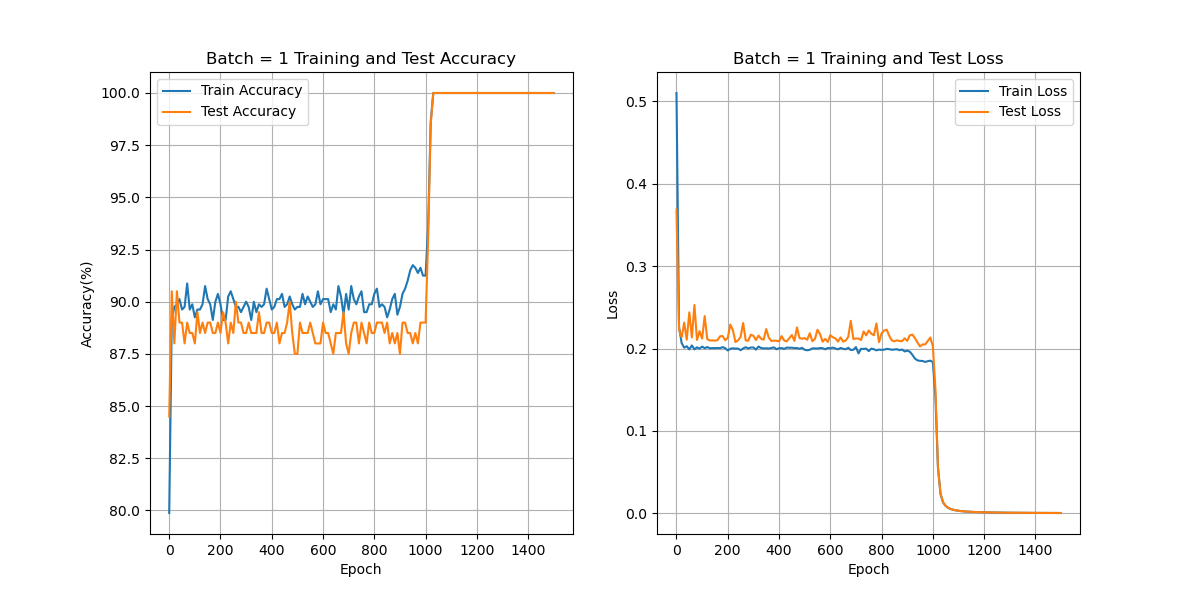
\includegraphics[width=0.85\textwidth]{img/Part2/curve_batch_1.png}
    \caption{SGD}
    \label{fig:p2batch1}
\end{figure}

\begin{figure}[!htbp]
    \centering
    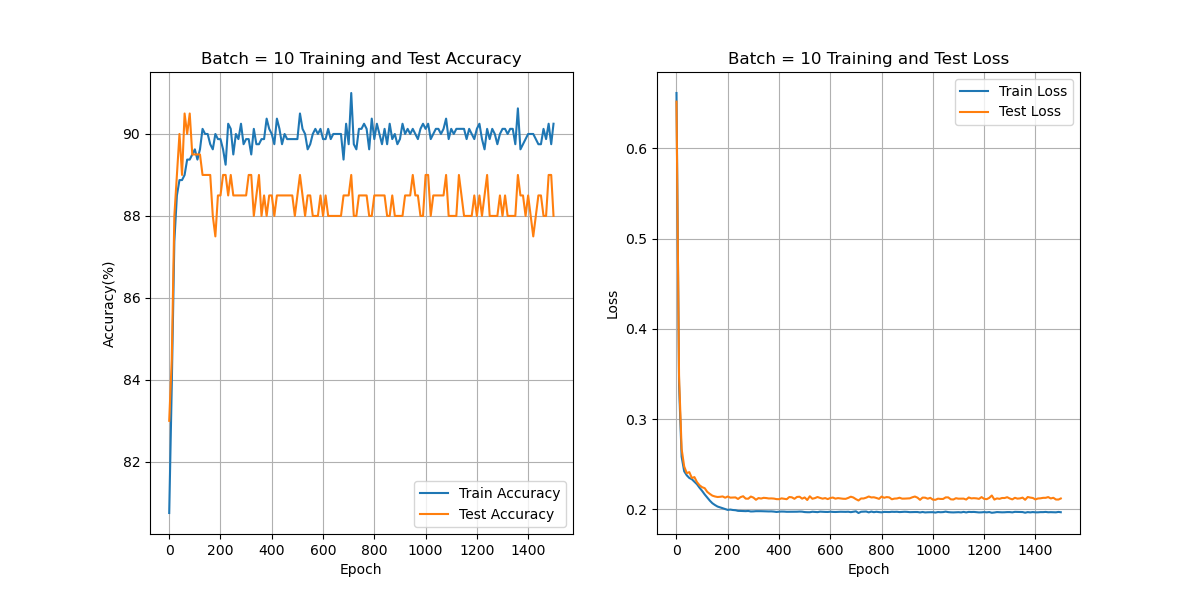
\includegraphics[width=0.85\textwidth]{img/Part2/curve_batch_10.png}
    \caption{BGD size 10}
    \label{fig:p2batch10}
\end{figure}

\begin{figure}[!htbp]
    \centering
    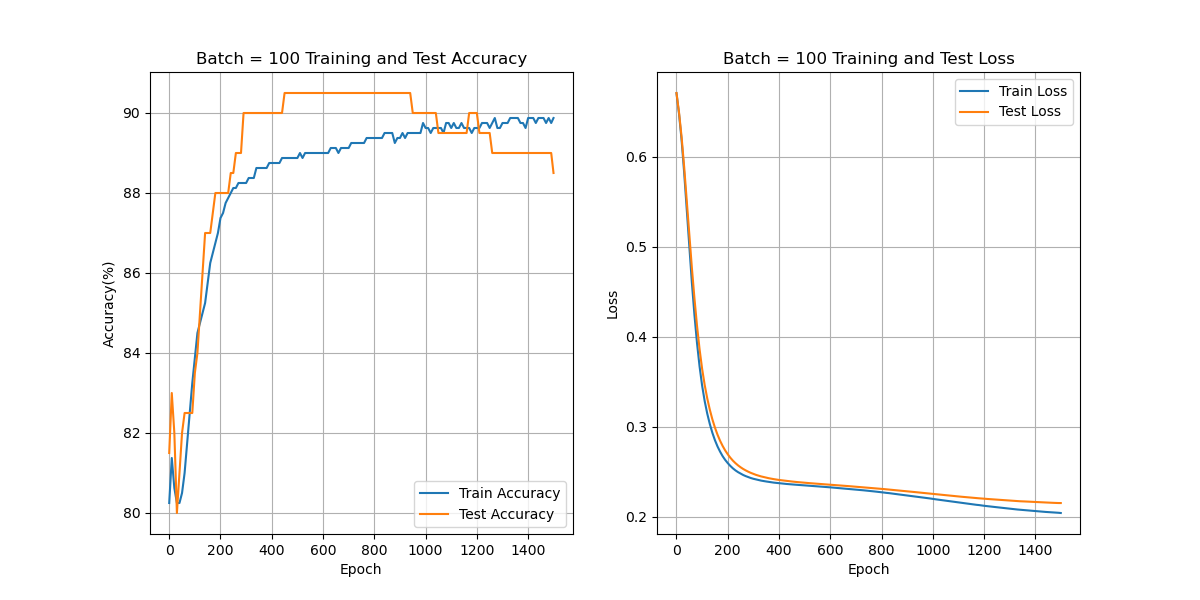
\includegraphics[width=0.85\textwidth]{img/Part2/curve_batch_100.png}
    \caption{BGD size 100}
    \label{fig:p2batch100}
\end{figure}

\begin{figure}[!htbp]
    \centering
    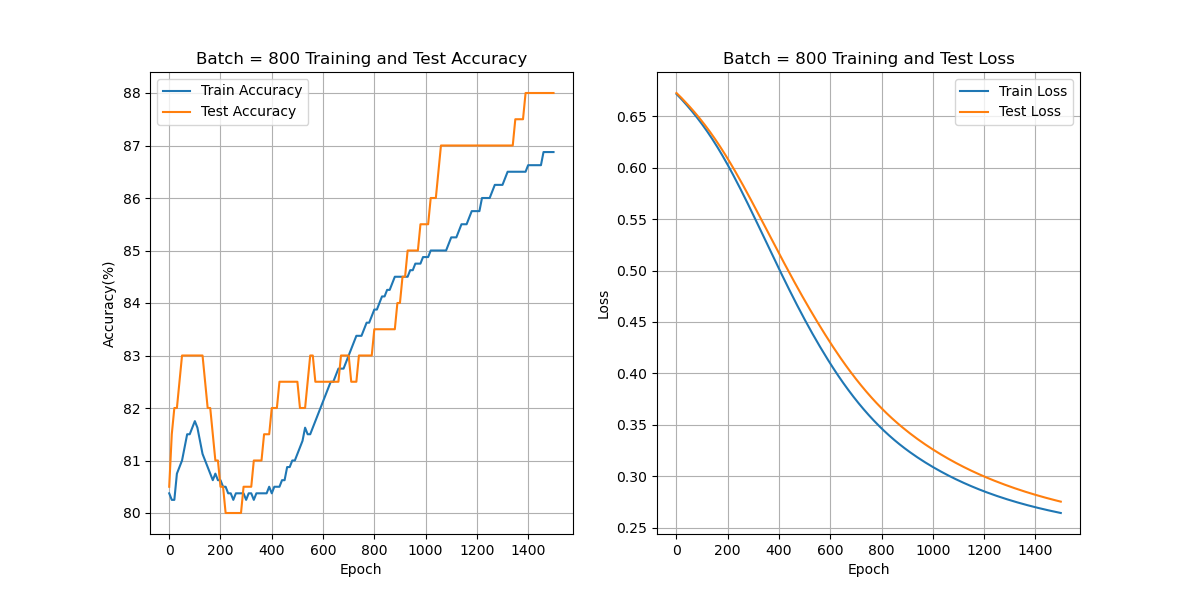
\includegraphics[width=0.85\textwidth]{img/Part2/curve_batch_800.png}
    \caption{BGD size 800}
    \label{fig:p2batch800}
\end{figure}

\subsection{Results and Analysis}

Because I mainly focused on the analysis of SGD and BGD, I did not consider changing other default parameters in this part. They maintain consistent values.

\subsubsection{Characteristic Analysis}

In general, SGD and smaller batche sizes mean faster training: less data is involved in each iteration, making iterations faster. But in this Assignment, epoch is given, which means that although the data in each iteration becomes less, we need more iterations to complete the traversal of the entire sample. requirements are reduced, this will lead to the loss of parallel computing opportunities for large matrices, a decrease in the overall utilization of the computing core, and a significant increase in time consumption.

\subsubsection{SGD Analysis}

For SGD, it declines very quickly in each epoch: in each epoch, it iterates 800 times and updates the weights 800 times. At first glance, it has more opportunities for decline than large batches. However, we can see that after experiencing a rapid decline in the initial stage, its loss curve has experienced great fluctuations.

This is because each time gradient descent is performed on a single sample, it is easy to fall into a local optimal. In the fitting of a single sample, the individual samples may interfere with each other (e.g, the previous one sample updates a certain weight value by +1, and the latter one then updates this value by -1), resulting in a loss that cannot be reduce at each epoch, even lead to an increase in loss.

However, under the large number of iterations, SGD finally found an opportunity to rapidly increase the model fitting degree. Therefore, after two rapid fittings to the training set, the loss of the model has been greatly reduced and the accuracy has reached a relatively good state.

\subsubsection{BGD Analysis}

Different from the overview in the previous section, in this section I will highlight the impact of batch size on training characteristics in several aspects.

\textbf{Attention: everything is based on the epoch is given.}

\begin{itemize}
    \item \textbf{Training speed}: As the batch size continues to increase, the number of iterations required begins to decrease, which makes the training speed significantly faster.
    \item \textbf{Loss}: As the batch size increases, it is easier for the model to find the global optimal point in each iteration update. Although the loss decreases less for each epoch (because the number of updates becomes less), the model can easily find the global optimal point of gradient descent, which makes the loss decrease more smoothly with almost no fluctuations.
    \item \textbf{Accuracy}: As the batch size becomes larger, the final accuracy limit is not as good as SGD because the number of iterations becomes smaller. However, the training accuracy of the model is still rising steadily. If there are more iteration opportunities, I believe it can reach a higher level.
    \item \textbf{Overfitting}: This is one of my observations: although the training accuracy of BGD with large batch size is constantly getting higher, its accuracy on the test set is not necessarily the same. BGD has lower generalization ability than SGD, and the risk of overfitting to the training set will be higher.
\end{itemize}

\subsubsection{Additional Analysis}

The appendix includes more mini-BGD test data and is updated with each iteration. I can learn more about the characteristics of each iteration of SGD and mini-BGD: the overall convergence speed is fast, but the fluctuation range is really large.

\subsection{Simple Conclusion}

In this part, I implemented a MLP. I learned about the hidden layer, softmax layer and cross-entropy loss function, and their corresponding forward propagation and back propagation formulas. In the comparison of different batch sizes, we learned about the various characteristics and principles hidden in training.

\newpage

\begin{appendix}

\section{Extra Pictures}

\begin{figure}[!ht]
  \centering
  \begin{subfigure}[b]{0.5\textwidth}
    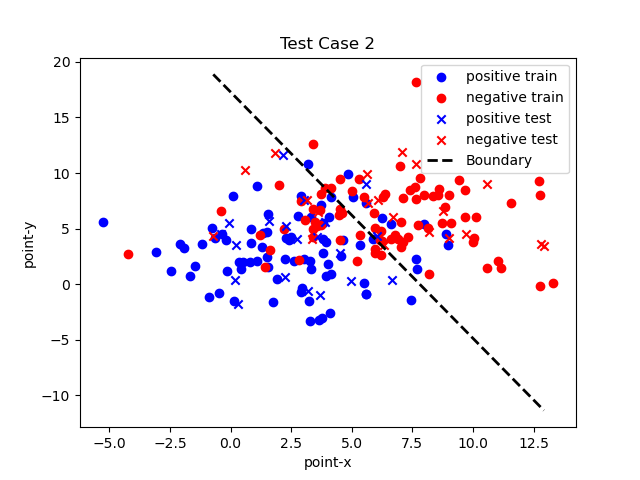
\includegraphics[width=\textwidth]{img/Part1/test2_data.png}
    \caption{Test case 2 Data}
  \end{subfigure}
  \begin{subfigure}[b]{1\textwidth}
    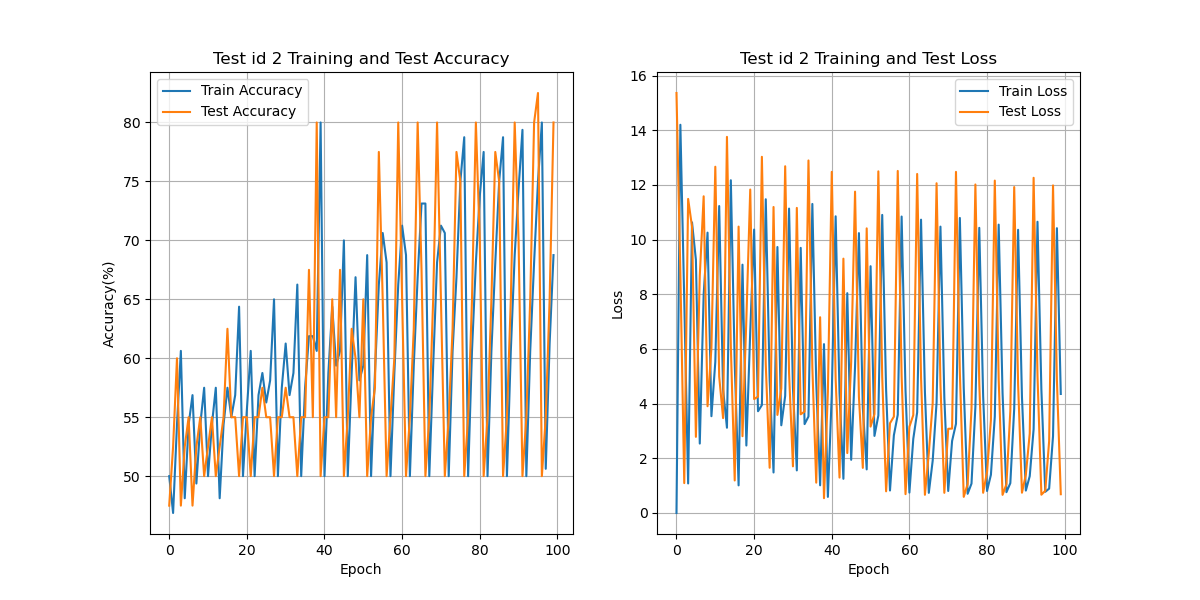
\includegraphics[width=\textwidth]{img/Part1/test2_curve.png}
    \caption{Test case 2 Accuracy and Loss}
  \end{subfigure}
  \caption{Part 1 Test Case 2}
  \label{fig:p1test2}
\end{figure}

\begin{figure}[!ht]
  \centering
  \begin{subfigure}[b]{0.5\textwidth}
    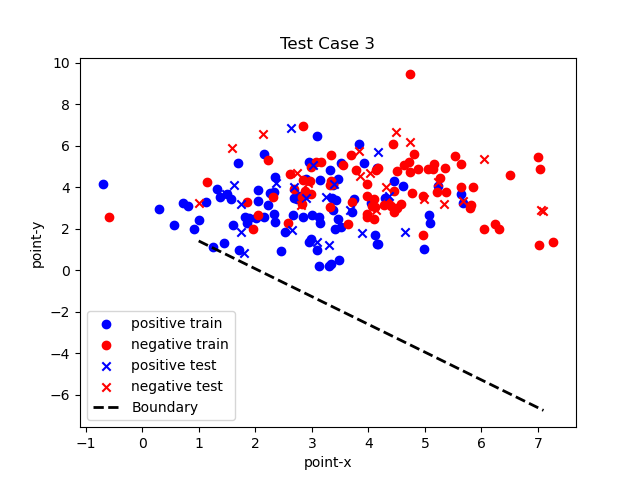
\includegraphics[width=\textwidth]{img/Part1/test3_data.png}
    \caption{Test case 3 Data}
  \end{subfigure}
  \begin{subfigure}[b]{1\textwidth}
    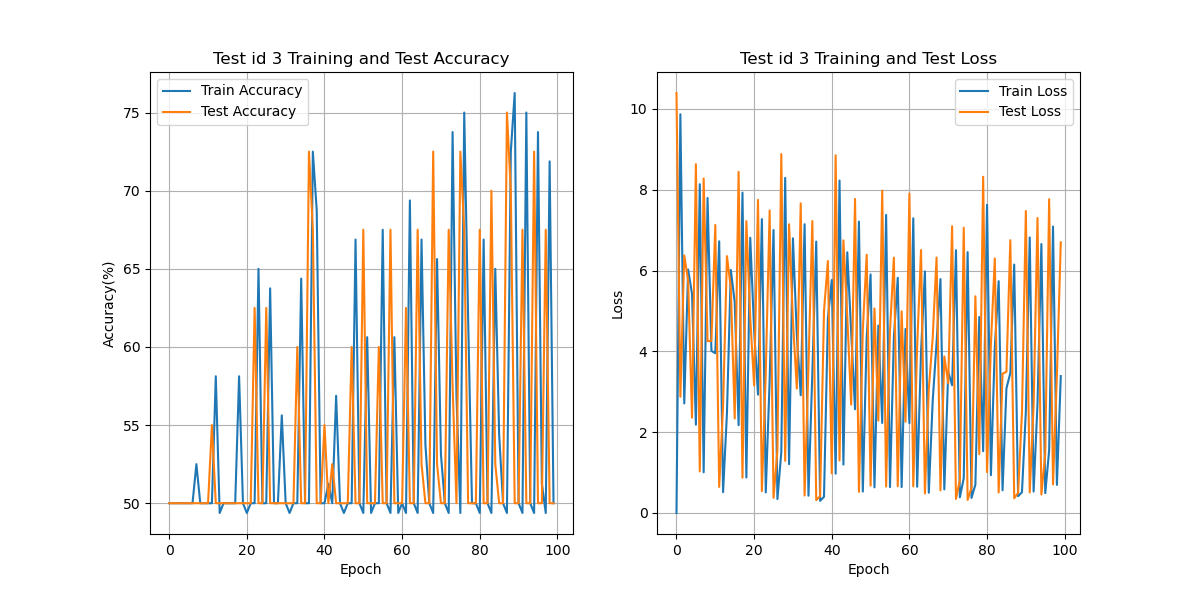
\includegraphics[width=\textwidth]{img/Part1/test3_curve.png}
    \caption{Test case 3 Accuracy and Loss}
  \end{subfigure}
  \caption{Part 1 Test Case 3}
  \label{fig:p1test3}
\end{figure}

\begin{figure}[!htbp]
    \centering
    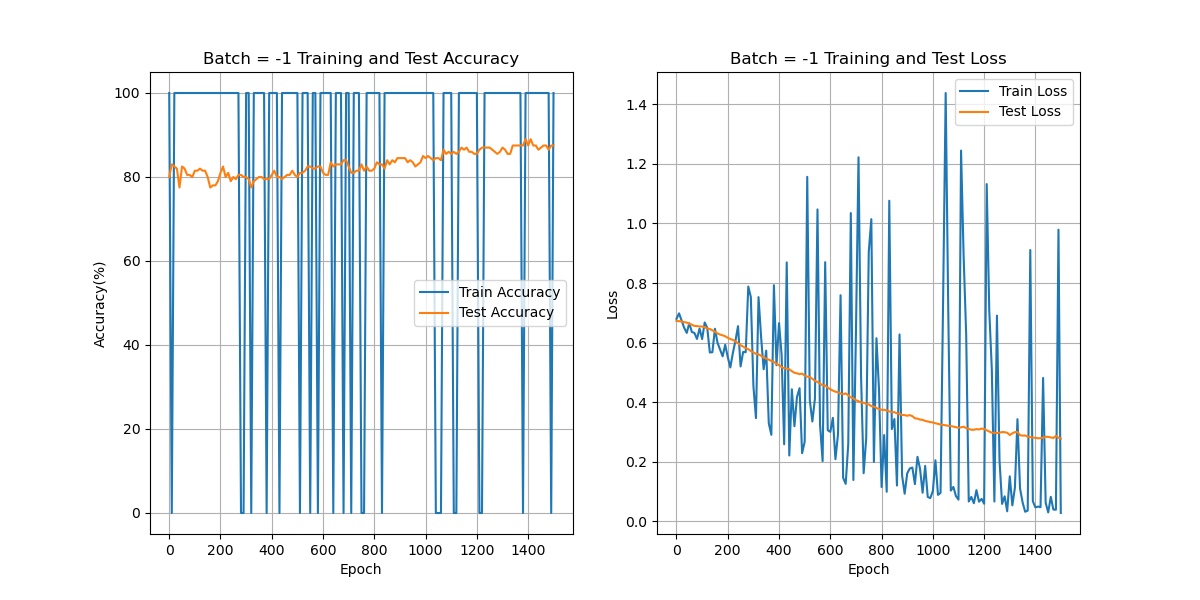
\includegraphics[width=0.9\textwidth]{img/Part2/curve_batch_-1.png}
    \caption{Mini Batch Size 1 with 1500 Iterations}
    \label{fig:p2batch-1}
\end{figure}


\begin{figure}[!htbp]
    \centering
    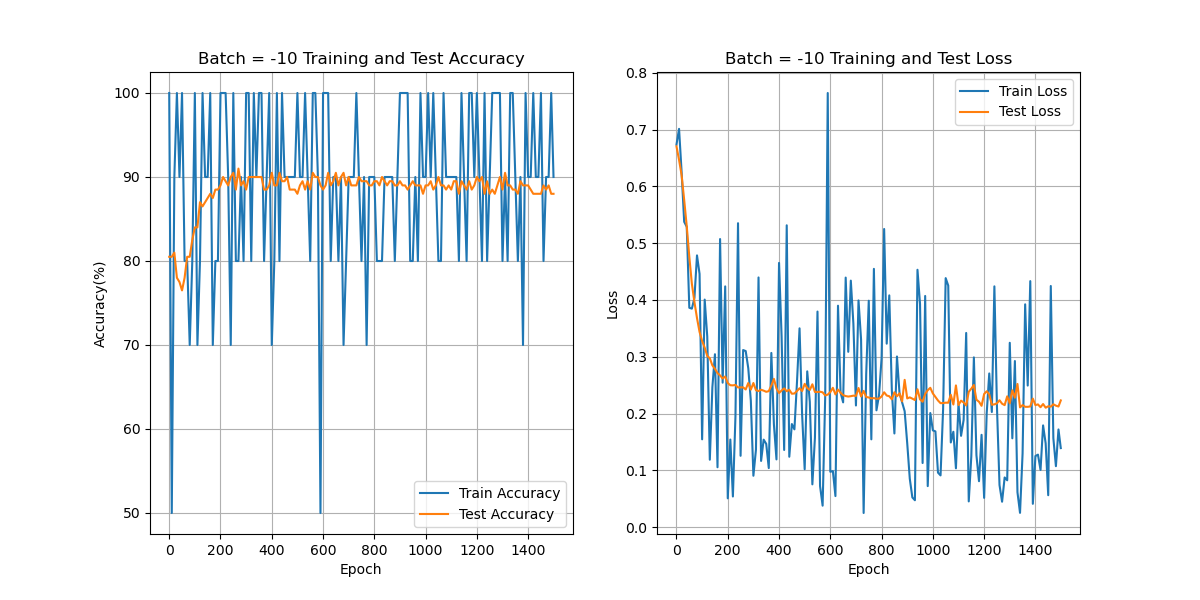
\includegraphics[width=0.9\textwidth]{img/Part2/curve_batch_-10.png}
    \caption{Mini Batch Size 10 with 1500 Iterations}
    \label{fig:p2batch-10}
\end{figure}


\begin{figure}[!htbp]
    \centering
    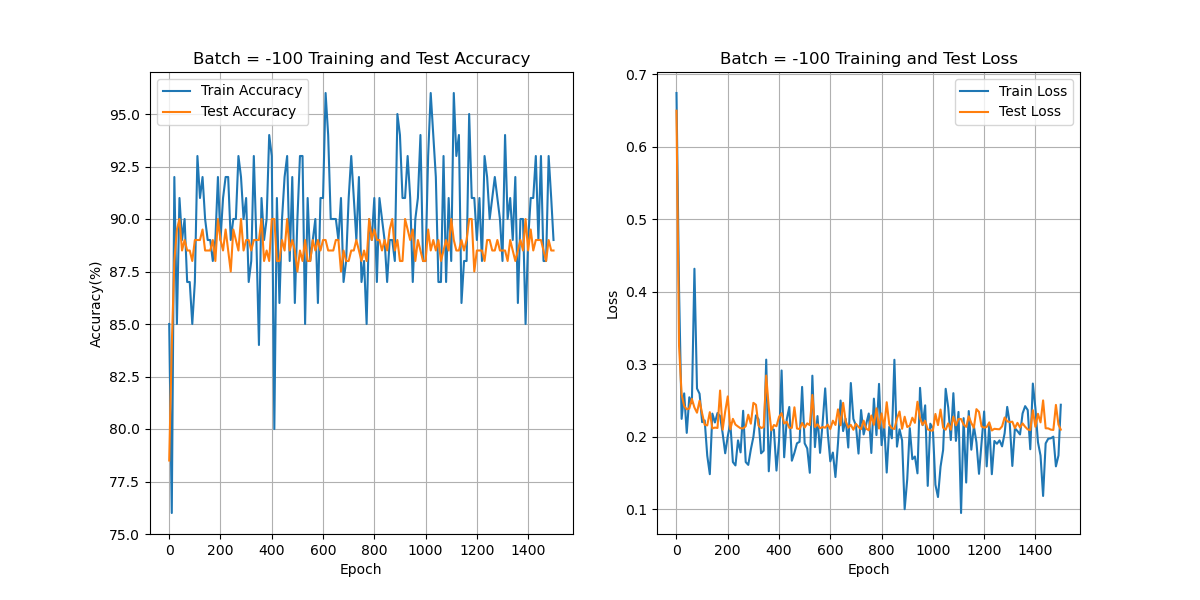
\includegraphics[width=0.9\textwidth]{img/Part2/curve_batch_-100.png}
    \caption{Mini Batch Size 100 with 1500 Iterations}
    \label{fig:p2batch-100}
\end{figure}


\end{appendix}

\end{document}

